\section{Event-based Multispectral and Depth Sensing}
This section introduces the basics of an event camera in \Sec \ref{sec:eventcam} principles of depth sensing (\Sec \ref{sec:esl}) and multispectral imaging (\Sec \ref{sec:emi}).

\subsection{Event Camera}
\label{sec:eventcam}
Event-cameras are novel, bio-inspired sensors that asynchronously measure \emph{changes} (i.e., temporal contrast) in illumination at every pixel, at the time they occur \cite{Lichtsteiner08ssc,Suh20iscas,Finateu20isscc, Posch11ssc}.
In particular, an event camera generates an event $e_k = (\mathbf{x}_k,t_k,p_k)$ at time $t_k$ when the difference of logarithmic brightness at the same pixel $\mathbf{x}_k=(x_k,y_k)^\top$  reaches a predefined threshold $C$:
\begin{equation}
\label{eq:egm}
    L(\mathbf{x_k},t_k) - L(\mathbf{x_k},t_k-\Delta t_k) = p_k C,
\end{equation}
where $p_k \in \{-1,+1\}$ is the sign (or polarity) of the brightness change, 
and $\Delta t_k$ is the time since the last event at the pixel $\mathbf{x}_k$. The result is a sparse sequence of events which are asynchronously triggered by illumination changes.

\subsection{Active illumination and event camera}
Significant literature on event-based vision has assumed brightness constancy, where events are only generated due to relative motion between the camera and scene.
However, the presence of active illumination source changes the event generation model.

%Introduce the project-based illumination change.
% \subsection{Event-based Depth Sensing}
% \label{sec:esl}
% This section introduces the basic considerations of event camera-projector setup and presents the optimization approach to depth estimation using spatio-temporal consistency between the signals used on the event camera and the projector.
% It is based on the Event-based Structured Light system introduced in \cite{Muglikar203DV}.
% The setup consists of a laser scanning projector and an event camera.
% The projector is a point scanning laser that scans in a raster scanning pattern.
% The change in illumination caused due to the moving light source triggers events in the event camera.
% The timestamps of the events are used to triangulate the 3D point.
% This leads to higher spatial accuracy of the depth, as the scene is densely scanned.
% It also performs better than frame-based baselines due to higher invariance to scene reflectivity.
It was shown in \cite{Matsuda18ICCP}, that the change in illumination ($\delta I$) observed by the event camera, caused by the projector $I_p$ shining light onto a point with reflectivity $T$, illuminated by ambient light $I_a$ is as follows:
\begin{equation}
    \delta I = log (\frac{I_p + I_a}{I_a})\\
             %=  log ((I_p + I_a) \times T) - log(I_a \times T) \\
\end{equation}
In this setting, according to the equation above, the generation of events no longer depends on the scene reflectivity.
This results in improved performance in terms of depth, for scenes containing varying reflectivity.
Unfortunately, the independence from reflectivity would also suggest that it is impossible to be recovered.
In the next section we show how it is nonetheless possible to recover relative scene reflectivity in this setup.

\subsection{Event-based Spectral Imaging}
\label{sec:emi}
In an ideal sensor, the measured change of intensity due to projector illumination is independent of the scene reflectivity.
However, non-idealities of the sensor architecture enable us to capture the scene reflectance:
The output of the photo-diode at each pixel, which measures the incoming light intensity, is not connected directly to the comparator circuit which measures change and creates events.
Its voltage is first passed through an amplifier and a source follower circuit. 
The source follower constantly tries to match the voltage of its source, which is the (amplified) signal from the photoreceptor.
The speed at which it can reach the target voltage is determined by the sf bias current and the magnitude of the signal voltage, which depends on the incoming light intensity.
This relationship between the light intensity and source-follower voltage introduces a dependence on scene reflectivity.
Our methods uses the fact that the bandwidth of the source follower in each pixel depends on the absolute intensity that its photoreceptor receives.
It implies that pixels corresponding to darker regions of a scene will result in a slower response (resulting in a lower rate of events) whereas brighter regions will respond faster (resulting in a larger event rate).

% \subsubsection{Intensity Reconstruction}
% Our setup combines an event camera with a projector. 
% The projector flashes the scene 60 times per second. 
% This flashing induces events in the event camera.
% To capture spectral images, we project all the spectral bands of light sequentially. 

% \newline
% \newline
% To reconstruct intensities, we make use of the variable bias currents in the event camera's pixel circuit.
% During each flash of the projector, the camera produces binary information at each pixel: Either events were generated or not.
% If and only if an event has been generated, the measured brightness change has exceeded the contrast threshold according to equation \ref{eq:contrastEquation}.
% \newline
% \begin{equation}
%     \label{eq:contrastEquation}
%     |log(I) - log(I_{ref})| > c
% \end{equation}
% \newline
% Here, $log(I)$ represents the signal generated by the logarithmic photo receptor in the DVS circuit \cite{DVSBiases}, $log(I_{ref})$ is the reference brightness, and $c$ is the contrast threshold. For every flash an event of both positive and negative polarity will be created. In our method we only consider positive polarity events, in which case the signal will be the brightness when the light is turned on while the reference will be the ambient brightness.
% According to equation \ref{eq:contrastEquation}, the camera measures relative changes of intensity.
% However, the DVS circuit output does have a dependence on the absolute pixel intensity resulting from multiple sources.
% One particular such dependence comes from the source follower. It bridges the logarithmic intensity measured by the photoreceptor with the comparator circuit responsible for generating events (Figure \ref{fig:eventCircuit}).
% Its purpose is to reduce noise events by smoothing out the signal generated by the photoreceptor. However, when paired with a fast periodic signal, its amplitude is determined by the absolute signal intensity. This behavior is qualitatively illustrated in Figure \ref{fig:sourceFollower}.

\begin{figure}
    \centering
    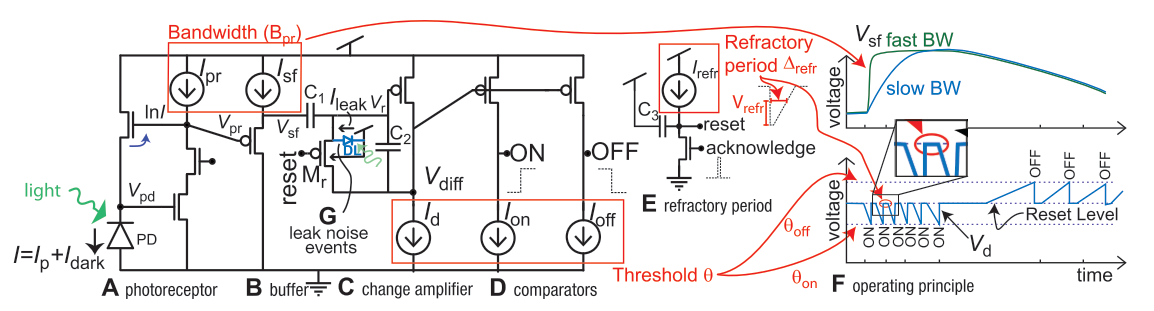
\includegraphics[width=\linewidth]{resources/images/intensity-estimation/DVSCircuit.png}
    \caption[Schematic of the DVS Pixel Circuit]{Schematic of the DVS Pixel Circuit taken from \cite{DVSBiases2023}. It can be divided into a photoreceptor part (\textbf{A}), a source follower part (\textbf{B}) and a comparator part (\textbf{C} and \textbf{D})}
    \label{fig:eventCircuit}
\end{figure}

\begin{figure}
    \centering
    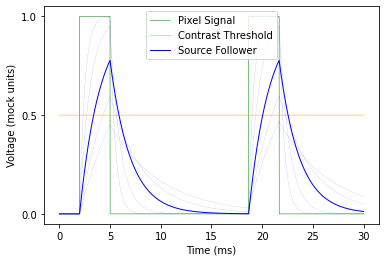
\includegraphics[width=.5\textwidth]{resources/plots/intensity-estimation/source_follower.png}
    \caption[Qualitative Simulation of the Source Follower with an Oscillating Signal]{The simulation demonstrates how a change in the source follower bandwidth can regulate the observed signal amplitude downstream. Responses for different follower gains are shown as dotted lines.}
    \label{fig:sourceFollower}
\end{figure}

% Our method then captures pixel-wise intensity measurements as follows:
% We repeatedly flash the scene at different contrast thresholds.
% With each flash we gain increasingly higher resolution estimates of the measured pixel intensity through event generation.
% The final intensity of the pixel is estimated using the last contrast threshold at which an event was still generated at its coordinates \ref{fig:scanning}. The accuracy of the estimate depends on the density at which the measurements were taken and the ambient lighting.
% \begin{figure}
    \centering
    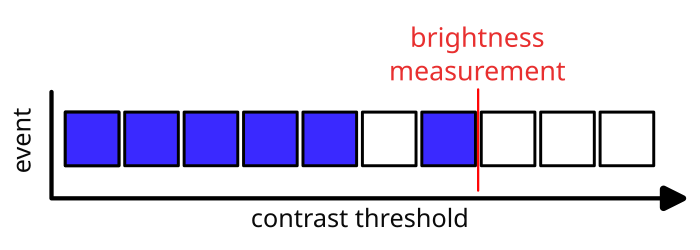
\includegraphics[width=.9\textwidth]{chapters/papers/ED/resources/plots/intensity-estimation/scanning.png}
    \caption{Schematic of the capture method. Events are shown in blue, no events are shown in white. The pixel's brightness is measured as the highest contrast threshold at which an event was received.}
    \label{fig:scanning}
\end{figure}

% \subsubsection{Linearization of measurements}
% The raw measurements are logarithmic with respect to the real light intensity values. A mapping between measurements is thus needed to extract a linear intensity image from the voltage readings extracted from the previous step.
% For this we fit a simple exponential function to the measured brightness values (Figure \ref{fig:chart_brightness_curves}).
